
\documentclass[aspectratio=169]{beamer}
\usetheme{metropolis}           % Use metropolis theme
\usepackage[utf8]{inputenc}
\usepackage{graphicx}
\usepackage{eso-pic}
\usepackage{graphics}
\usepackage{tikz}
\usepackage[export]{adjustbox}
\usepackage{multicol}
\usepackage{listings}
\usepackage{helvet}
\usepackage{booktabs}
\usepackage{threeparttable}
\usepackage{fontspec}
\usepackage{hyperref}
\hypersetup{urlcolor=DarkBlue}

\title{Topic 4 - Track 1 \newline Real Time Data Quality Checks}
\date{\today}
\author{Author of Session here!} % Name of author(s) of session here
\institute{Development Impact Evaluation (DIME) \newline The World Bank }
\setbeamercolor{background canvas}{bg=white}	% Sets background color

% The below command places the World Bank logo and DIME logo to the right corner
\titlegraphic{%
	\begin{picture}(0,0)
	\put(330,-180){\makebox(0,0)[rt]{
\includegraphics[width=3cm]{../../img/WB_logo}}}
	\end{picture}%
	\begin{picture}(0,0)
	\put(390,-180){\makebox(0,0)[rt]{
\includegraphics[width=1.5cm]{../../img/i2i}}}
	\end{picture}%
}

%%% Section page with picture of Light bulb
\makeatletter
\defbeamertemplate*{section page}{mytheme}[1][]{
	\centering
	\begin{minipage}{22em}
		\raggedright
		\usebeamercolor[fg]{section title}
		\usebeamerfont{section title}
		\par
		\ifx\insertsubsectionhead\@empty\else%
		\usebeamercolor[fg]{subsection title}%
		\usebeamerfont{subsection title}%
		\fi
		\ifstrempty{#1}{}{%
			\includegraphics[width=100mm, height=60mm]{#1}%
		}
		\insertsectionhead\\[-1ex]
		\insertsubsectionhead
		\usebeamertemplate*{progress bar in section page}

	\end{minipage}
	\par
	\vspace{\baselineskip}
}
\makeatother

%%% Define a command to include picture in section,
%%% make section, and revert to old template
\newcommand{\sectionpic}[2]{
	\setbeamertemplate{section page}[mytheme][#2]
	\section{#1}
	\setbeamertemplate{section page}[mytheme]
}

\usepackage{fancyvrb} % Allows customization of verbatim environments
%Fancyvrb docs: http://mirrors.ibiblio.org/CTAN/macros/latex/contrib/fancyvrb/doc/fancyvrb-doc.pdf
\fvset{fontsize=\scriptsize} % The font size of all verbatim text can be changed here

%So we can use option FloatBarrier, which is similar to [H] but is an
%alternative solition when the algorithm can't solce [H] as too many
%settings are going on. [H] seems to get stuck in infinite loop
%https://tex.stackexchange.com/questions/2275/keeping-tables-figures-close-to-where-they-are-mentioned
\usepackage{placeins}
\newcommand{\codeexample}[2]{
	\begin{figure}
		\VerbatimInput[
		framesep=3mm,
		frame=lines, % line above and below code section
		numbers=left, %Line number
		label= #1, %name of code section
		baselinestretch=0.90, %Use line space more similat to line space in code editors
		]{#2} %Write the relative file path and the name of the file to be included
	\end{figure}
	\FloatBarrier
}

%% The below command creates the ligh bulb logos in the top right corner of the
\begin{document}

	{
		\usebackgroundtemplate{
\includegraphics[height=55mm, right]{../../img/top_right_corner.pdf}}
		\maketitle
	}

%%%%%%%%%%%%%%%%%%%%%%%%%%%%%%%%%%%%%%%%%%% heading of section 1
\begin{frame}{Objectives}
	\begin{itemize}
		\item Duplicates
		\begin{itemize}
			\item Run a prepared file using \texttt{ieduplicates} command and understand the output
			\item \texttt{Purpose:} Make sure you can identify the respondent while the enumerator still remember the interview
		\end{itemize}
		\item Survey Log / Progress Report
		\begin{itemize}
			\item List the number of completed interviews
			\item \texttt{Purpose:} Make sure we are making enough progress to complete sample before money runs out
		\end{itemize}
		\item High Frequency Checks (HFC)
		\begin{itemize}
			\item Download and use IPA's framework for HFCs
			\item \texttt{Purpose:} Make sure we are collecting data without a lot of errors reducing the quality of the data
		\end{itemize}
	\end{itemize}
\end{frame}

%%%%%%%%%%%%%%%%%%%%%%%%%%%%%%%%%%%%%%%%%%%
\sectionpic{Duplicates}{../../img/section_slide}

\begin{frame}{Why do we have duplicates?}
	\begin{itemize}
		\item To develop a quick but still secure way of dealing with any issue, we must first have a model for understanding the reasons that cause this issue
		\item Once we have a good model of the reasons for the issue, we will be able to develop a good methodology for how to solve the issues
		\item What type of reasons do we have for the duplicates in the ID variable we find in primary data?
	\end{itemize}
\end{frame}

\begin{frame}{Why do we have duplicates?}
	\begin{itemize}
		\item Type 1 - Double submissions of same observation and the same data
		\begin{itemize}
			\item First upload from tablet not complete due to bad internet
		\end{itemize}
		\item Type 2 - Double submissions of same observation but with modified data.
		\begin{itemize}
			\item Answers modified after submission, and then re-submitted
			\item Bad practice, more transparent to write correction in a do-file
			\item Many survey software have features preventing this.
		\end{itemize}
		\item Type 3 - Incorrectly assigned ID. Two respondents are given the same ID
		\begin{itemize}
			\item Typo in field when entering respondent ID
		\end{itemize}
	\end{itemize}
\end{frame}

\begin{frame}{How can we identify the types of duplicates?}
	\begin{itemize}
		\item Type 1 - Double submissions of same observation and the same data
		\begin{itemize}
			\item Few variables differs between the duplicates and differences are in submission data
			\item (\texttt{submission data} = submission time, submission ID, file attachment name etc.)
		\end{itemize}
		\item Type 2 - Double submissions of same observation but with modified data.
		\begin{itemize}
			\item Some variables differs between the duplicates and some of them are in observation data
			\item (\texttt{observation data} = age of respondent, professional occupancy, marital status, crops grown, what did you eat yesterday etc.)
		\end{itemize}
		\item Type 3 - Incorrectly assigned ID. Two respondents are given the same ID
		\begin{itemize}
			\item Many variables differs between the duplicates and many of the differences are in observation data
		\end{itemize}
	\end{itemize}
\end{frame}

\begin{frame}{ieduplicates}
	
	Wouldn't it be great if there was an command in Stata that would identify all duplicates and provide you with the information needed to determine which type it is?

	\begin{itemize}
		\item We have written: \texttt{ieduplicates}
		\begin{itemize}
			\item Part of the \texttt{ietoolkit} package. Installation \texttt{ssc install ietoolkit}
			\item Used in Stata but generates a report in Excel that team members not proficient in Stata can interact with
			\item The report is interactive, so you write your corrections in the Excel report, and the command will then apply those corrections
			\item Returns the data without the duplicates until they are solved
		\end{itemize}
	\end{itemize}
\end{frame}

\begin{frame}{ieduplicates - output}
	\begin{figure}
		\centering
		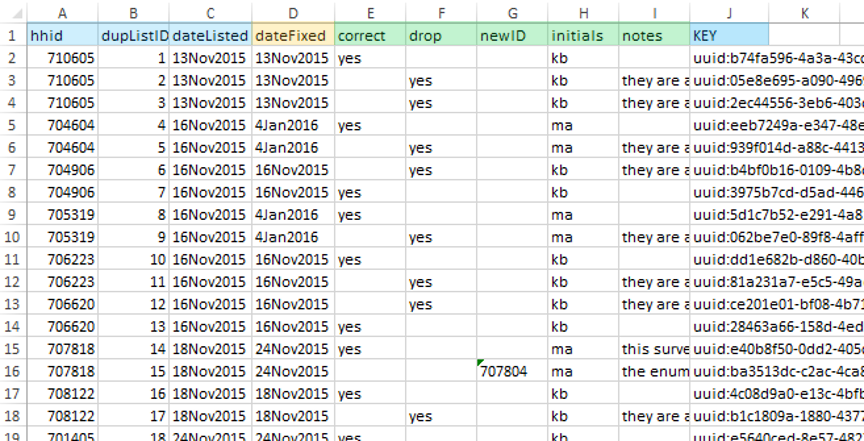
\includegraphics[width=.9\linewidth]{img/ieduplicates-output.png}
	\end{figure}
\end{frame}

\begin{frame}{ieduplicates - output}
	Attend the hands-on session on \texttt{ieduplicates} and \texttt{ietestform} to learn the details on how to best use \texttt{ieduplicates}. We will introduce some new features that were released only last month!
\end{frame}

%%%%%%%%%%%%%%%%%%%%%%%%%%%%%%%%%%%%%%%%%%%
\sectionpic{Survey Log}{../../img/section_slide}



\begin{frame}{3. Survey Log}
	\begin{itemize}
		\item Make sure to keep records in the field that is updated very day with how many interviews that were completed
		\item Make sure that the number of observations on the server matches these records.
		\item Purpose:
		\begin{itemize}
			\item Provide your team a quick overview of progress on the field
			\item Detect enumerators who are slacking
			\item Check balance if this is important for the survey (e.g. by gender)
		\end{itemize}
	\end{itemize}
\end{frame}


\begin{frame}{3. Survey Log}
	\begin{itemize}
		\item Exercise 2 – Practice checking survey progress. Assume you’ve verified that the server matches the field log, i.e. no submissions are missing.
	\end{itemize}
\end{frame}


\begin{frame}{4. Back checks}
	\begin{itemize}
		\item Purpose
		\begin{itemize}
			\item To monitor the quality of field work: Do some enumerators need extra support from supervisors?
			\item To understand whether your questionnaire accurately captures the key outcomes of your study: Do respondents understand the questions the way we intended to?
		\end{itemize}
		\item Best practices:
		\begin{itemize}
			\item ~ 10\% of surveys, 20\% in the first 2 weeks of field work
			\item Every team and every surveyor must be back checked
			\item The back check sample must include a proportional number of missing and replacement respondents.
			\item Selection of households for back checks must be random
		\end{itemize}
	\end{itemize}
\end{frame}

\begin{frame}{Selecting Back Check Questions}
	\begin{itemize}
		\item Type 1 variables
		\begin{itemize}
			\item Straightforward questions where we expect very little variation
			\item E.g. education level, marital status, occupation, has children
		\end{itemize}
		\item Type 2 variables
		\begin{itemize}
			\item Questions where we expect capable enumerators to get the true answer
		\end{itemize}
		\item Type 3 variables
		\begin{itemize}
			\item Questions that we expect to be difficult.
			\item Want to understand if these questions were interpreted in the field as intended
		\end{itemize}
		\item Identifying Respondent and Interview Information
		\begin{itemize}
			\item Check if we have the right person; if the interview took place \& when
		\end{itemize}
	\end{itemize}
\end{frame}

\begin{frame}{bcstats}
	\begin{itemize}
		\item \texttt{ssc install bcstats}
		\item Purpose:
		\begin{itemize}
			\item compares back check data and survey data, producing a data set of comparisons
			\item completes enumerator checks and stability checks for variables
		\end{itemize}
	\end{itemize}
\end{frame}

\begin{frame}{Using bcstats report to improve data quality}
	\begin{itemize}
		\item Type 1
			\begin{itemize}
				\item If >10\% discrepancies  - give surveyor a warning
				\item 20-30\% discrepancies - 2nd backcheck to determine who made errors
				\item If error is by surveyor  - audit 3 additional surveys by that surveyor in same week
				\item if 20-30\% discrepancies -  put him/her on probation
				\item >40\% discrepancies - 2nd backcheck to determine who made errors and maybe re-survey HH
				\item If surveyor made errors - re-survey HH \& audit all surveys done by surveyor in this batch
				\item If one more survey has 40\% discrepancies - fire surveyor immediately \& redo all his/her surveys with 20\% or more discrepancies
		\end{itemize}
	\end{itemize}
\end{frame}

\begin{frame}{Using bcstats report to improve data quality}
	\begin{itemize}
		\item Type 2
		\begin{itemize}
			\item >10\% discrepancies -> Consider re-training
			\item If one surveyor is responsible for more than 30\% of the errors in a single question, follow the steps for Type 1
		\end{itemize}
		\item Type 3
		\begin{itemize}
			\item Discuss >10\% with your survey team and your PIs.
			\item PIs may decide to edit survey or add additional rounds
		\end{itemize}
	\end{itemize}
\end{frame}

\begin{frame}{4. Backchecks}
	\begin{itemize}
		\item Exercise 3
		\begin{itemize}
			\item Install bcstats
			\item Learn how to use bcstats
			\item Distinguish between types of backcheck variables
			\item Explore bcstats output
		\end{itemize}
	\end{itemize}
\end{frame}

%%%%%%%%%%%%%%%%%%%%%%%%%%%%%%%%%%%%%%%%%%% Final thougts section
\begin{frame}{Conclusion}


\vspace{20mm}
For more information or further questions please contact:
\newline John Doe (\url{johndoe@worldbank.org}) \newline Mary Doe (\url{marydoe@worldbank.org})

\end{frame}

%%%%%%%%%%%%%%%%%%%%%%%%%%%%%%%%%%%%%%%%%%% The End
\sectionpic{Thank You!}{../../img/section_slide}






\end{document}
